%%%%%%%%%%%%%%%%%%%%%%%%%%%%%%%%%%%%%%%%%
% Short Sectioned Assignment
% LaTeX Template
% Version 1.0 (5/5/12)
%
% This template has been downloaded from:
% http://www.LaTeXTemplates.com
%
% Original author:
% Frits Wenneker (http://www.howtotex.com)
%
% License:
% CC BY-NC-SA 3.0 (http://creativecommons.org/licenses/by-nc-sa/3.0/)
%
%%%%%%%%%%%%%%%%%%%%%%%%%%%%%%%%%%%%%%%%%

%----------------------------------------------------------------------------------------
%	PACKAGES AND OTHER DOCUMENT CONFIGURATIONS
%----------------------------------------------------------------------------------------

\documentclass[paper=a4, fontsize=11pt]{scrartcl} % A4 paper and 11pt font size

\usepackage{graphicx}
\usepackage[T1]{fontenc} % Use 8-bit encoding that has 256 glyphs
\usepackage{fourier} % Use the Adobe Utopia font for the document - comment this line to return to the LaTeX default
\usepackage[english]{babel} % English language/hyphenation
\usepackage{amsmath,amsfonts,amsthm} % Math packages

\usepackage{lipsum} % Used for inserting dummy 'Lorem ipsum' text into the template

\usepackage{sectsty} % Allows customizing section commands
\allsectionsfont{\scshape} % Make all sections centered, the default font and small caps

\usepackage{fancyhdr} % Custom headers and footers
\pagestyle{fancyplain} % Makes all pages in the document conform to the custom headers and footers
\fancyhead{} % No page header - if you want one, create it in the same way as the footers below
\fancyfoot[L]{} % Empty left footer
\fancyfoot[C]{} % Empty center footer
\fancyfoot[R]{\thepage} % Page numbering for right footer
\renewcommand{\headrulewidth}{0pt} % Remove header underlines
\renewcommand{\footrulewidth}{0pt} % Remove footer underlines
\setlength{\headheight}{13.6pt} % Customize the height of the header

\numberwithin{equation}{section} % Number equations within sections (i.e. 1.1, 1.2, 2.1, 2.2 instead of 1, 2, 3, 4)
\numberwithin{figure}{section} % Number figures within sections (i.e. 1.1, 1.2, 2.1, 2.2 instead of 1, 2, 3, 4)
\numberwithin{table}{section} % Number tables within sections (i.e. 1.1, 1.2, 2.1, 2.2 instead of 1, 2, 3, 4)

\setlength\parindent{0pt} % Removes all indentation from paragraphs - comment this line for an assignment with lots of text

%----------------------------------------------------------------------------------------
%	TITLE SECTION
%----------------------------------------------------------------------------------------

\newcommand{\horrule}[1]{\rule{\linewidth}{#1}} % Create horizontal rule command with 1 argument of height

\title{	
\normalfont \normalsize
\textsc{Rice University, Department of Computer Science} \\ [25pt] % Your university, school and/or department name(s)
\horrule{0.5pt} \\[0.4cm] % Thin top horizontal rule
\huge Assignment 1, COMP 540 \\ % The assignment title
\horrule{2pt} \\[0.5cm] % Thick bottom horizontal rule
}

\author{Chen Zeng(cz39), Zhihui Xie(zx18)} % Your name

\date{\normalsize\today} % Today's date or a custom date

\begin{document}

\maketitle % Print the title

%----------------------------------------------------------------------------------------
%	PROBLEM 1
%----------------------------------------------------------------------------------------

\section{Background refresher}

\paragraph{\textbf{Solution 1}}
\begin{itemize}
	\item Plot the histogram of samples generated by a categorical distribution with probabilities [0.2,0.4,0.3,0.1].
    \\ \textbf{Answer}: Figure \ref{fig:categorical} shows the result.
	
 	\item Plot the univariate normal distribution with mean of 10 and standard deviation of 1.
    \\ \textbf{Answer}: Figure \ref{fig:univariate} shows the result.
 	
 	\item Produce a scatter plot of the samples for a 2-D Gaussian with mean at [1,1] and a covariance matrix [[1,0.5],[0.5,1]].
    \\ \textbf{Answer}: Figure \ref{fig:multiVariate} shows the result.
 	
 	\item Test your mixture sampling code by writing a function that implements an equal-weighted mixture of four Gaussians in 2 dimensions, centered at $ (\pm 1, \pm 1) $ and having covariance I. Estimate the probability that a sample from this distribution lies within the unit circle centered at (0.1, 0.2) and include that number in your writeup.
 	\\ \textbf{Answer}: The estimated probability is 0.18075.
 	
	\begin{figure}
 		\centering
 		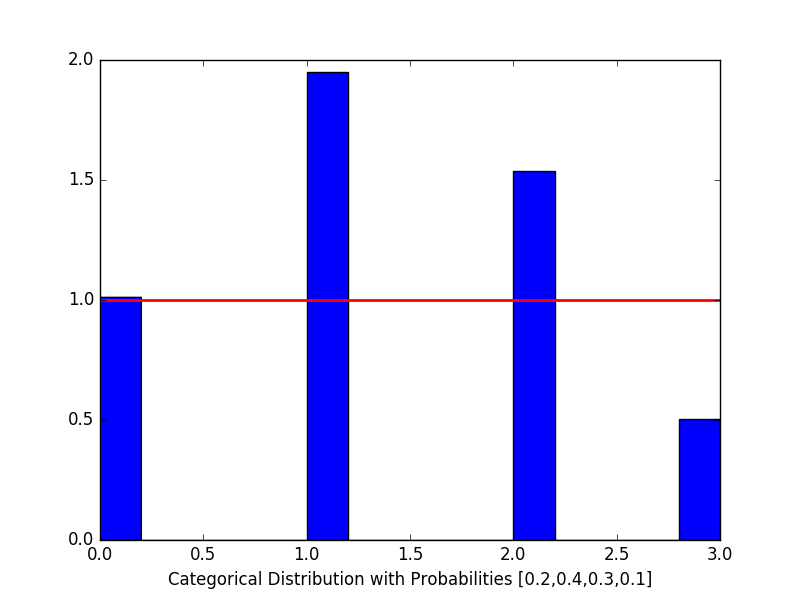
\includegraphics[scale=0.6]{Categorical.png}
 		\caption{Categorical Distribution}
 		\label{fig:categorical}
 	\end{figure}
 	\begin{figure}
 		\centering
 		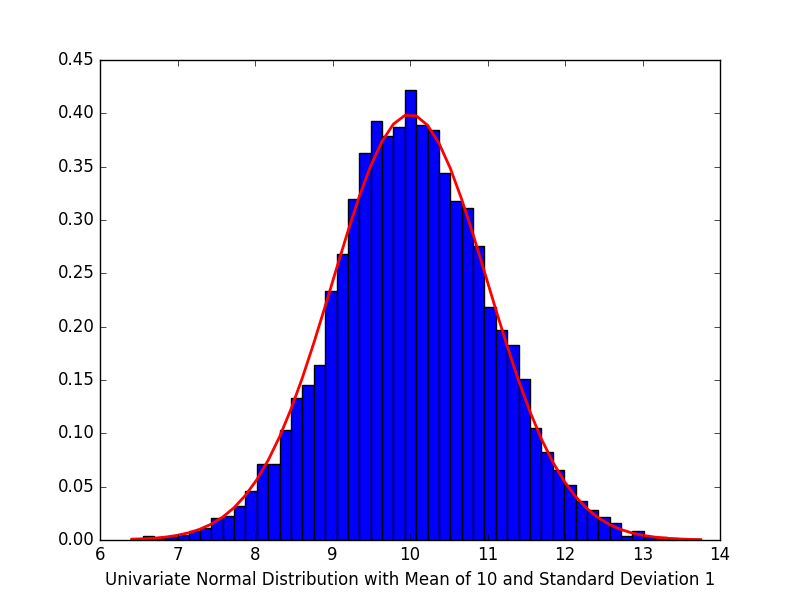
\includegraphics[scale=0.6]{UnivariateNormal.png}
 		\caption{Univariate Normal Distribution}
 		\label{fig:univariate}
 	\end{figure}
 	\begin{figure}
 		\centering
 		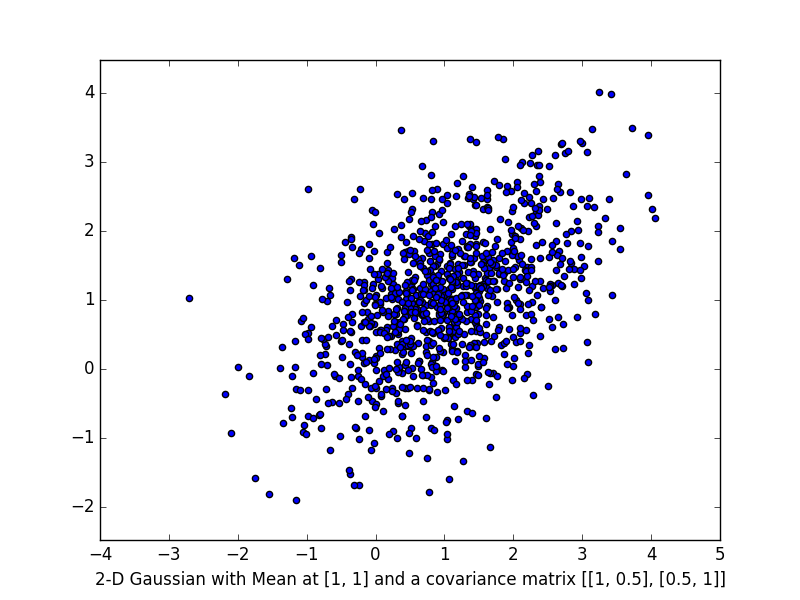
\includegraphics[scale=0.6]{MultiVariateNormal.png}
 		\caption{MultiVariate Normal Distribution}
 		\label{fig:multiVariate}
 	\end{figure}
\end{itemize}


\paragraph{\textbf{Solution 2}}
Here we suppose that there are two independent Poisson Random Variables and we define their moment-generating function as the following:
\begin{equation*}
X\sim P(\lambda _{1}), Y\sim P(\lambda _{2})
\end{equation*}
According to the properties of Poisson Random Variables, we can get:
\begin{equation*}
P\left ( X=x \right )= \frac{\lambda _{1}^{x}}{x!}e^{-\lambda _{1}}, P\left ( Y=y \right )= \frac{\lambda _{2}^{y}}{y!}e^{-\lambda _{2}}
\end{equation*}
Therefore, using the binomial formula and some transformation, we can get:
\begin{align*}
P\left ( X+Y=z \right )&= \sum_{x=0}^{z}\frac{\lambda _{1}^{x}}{x!}e^{-\lambda _{1}}\frac{\lambda _{2}^{z-x}}{\left ( z-x \right )!}e^{-\lambda _{2}}
\\ &=e^{-\left (\lambda _{1}+\lambda _{2} \right )}\sum_{x=0}^{z}\frac{\lambda _{1}^{x}}{x!}\frac{\lambda _{2}^{z-x}}{\left (z-x  \right )!}
\\ &=e^{-\left (\lambda _{1}+\lambda _{2} \right )}\frac{\left (\lambda _{1}+\lambda _{2}  \right )^{z}}{z!}
\end{align*}
According to the definition, $X+Y$ is also a Poisson random variable

\paragraph{\textbf{Solution 3}}
According to transformation, we can get:
\begin{align*}
p\left ( X_{1}=x_{1} \right )&=\int p\left ( X_{1}=x_{1},X_{0}=x_{0} \right )dx_{0}
\\ &=\int p\left ( X_{0}=x_{0} \right )p\left ( X_{1}=x_{1} |X_{0}=x_{0} \right)dx_{0}
\\ &=\alpha _{0}\alpha \int exp\left ( -\frac{1}{2}\left ( \frac{\left ( x_{0}-\mu _{0} \right )^{2}}{\sigma ^{2}_{0}}+ \frac{\left ( x_{1}-x_{0} \right )^{2}}{\sigma^{2} }\right ) \right )dx_{0}
\\ &=\frac{\alpha _{0}\alpha }{A}exp\left ( -\frac{1}{2}\frac{\left ( x_{1}-\mu _{0} \right )^{2}}{\sigma^{2}+\sigma _{0}^{2}} \right )
\end{align*}
Here $A$ is a constant. At the same time, according to the given condition we can know:
\begin{align*}
p\left ( X_{1}=x_{1} \right )=\alpha _{1}exp\left ( -\frac{1}{2}\frac{\left ( x_{1}-\mu _{1} \right )^{2}}{\sigma _{1}^{2}} \right )
\end{align*}
Therefore, we can get the relations:
\begin{equation*}
\mu _{1}=\mu _{0}
\end{equation*}
\begin{equation*}
\sigma _{1}^{2}=\sigma^{2}+\sigma _{0}^{2}
\end{equation*}
\begin{equation*}
\alpha _{1}=\frac{\alpha _{0}\alpha }{A}=\alpha _{0}\alpha\int exp\left (-\frac{1}{2} \frac{x_{0}^{2}-2\left ( \frac{\sigma ^{2}\mu _{0}+\sigma _{0}^{2}x_{1}}{\sigma ^{2}+\sigma _{0}^{2}} \right )x_{0}+\left ( \frac{\sigma ^{2}\mu _{0}+\sigma _{0}^{2}x_{1}}{\sigma ^{2}+\sigma _{0}^{2}} \right )^{2}}{\sigma _{0}^{2}\sigma^{2} /\left ( \sigma ^{2}+\sigma _{0}^{2} \right )} \right )dx_{0}
\end{equation*}

\paragraph{\textbf{Solution 4}}
As for eigenvalues, we just need to solve:
\begin{equation*}
(13-\lambda)(4-\lambda)=10
\end{equation*}
And we can get the result:
\begin{equation*}
\lambda _{1}=3, \lambda _{2}=4
\end{equation*}
As for eigenvectors, there are two cases:
\\ when $\lambda _{1}=3$: $A-\lambda I=\begin{bmatrix}
 10& 5\\
 2& 1
\end{bmatrix}$, and the according eigenvector is $\begin{bmatrix}
1\\-2
\end{bmatrix}$
\\ when $\lambda _{2}=14$: $A-\lambda I=\begin{bmatrix}
 -1& 5\\
 2& -10
\end{bmatrix}$, and the according eigenvector is $\begin{bmatrix}
5\\1
\end{bmatrix}$

\paragraph{\textbf{Solution 5}}
As for $\left ( A+B \right )^{2}\neq A^{2}+2AB+B^{2}$, we get the following example:
\begin{equation*}
A=\begin{bmatrix}
 1&0 \\
 1&0
\end{bmatrix}, B=\begin{bmatrix}
 0&-1 \\
 0&-1
\end{bmatrix}
\end{equation*}
\\ As for $AB=0, A\neq 0, B\neq 0$, we get the following example:
\begin{equation*}A=\begin{bmatrix}
 0&0 \\
 0&1
\end{bmatrix}, B=\begin{bmatrix}
 1&0 \\
 0&0
\end{bmatrix}
\end{equation*}

\paragraph{\textbf{Solution 6}}
\begin{align*}
A^{T}A &=\left ( I-2uu^{T} \right )^{T}\left ( I-2uu^{T} \right )
\\ &=\left ( I-2uu^{T} \right )\left ( I-2uu^{T} \right )
\\ &=I-4uu^{T}+4uu^{T}u u^{T}
\\ &=I-4uu^{T}+4u\left (u^{T}u  \right )u^{T}
\\ &=I-4uu^{T}+4uu^{T}=I
\end{align*}

\paragraph{\textbf{Solution 7-1}}
$f\left ( x \right )=x^{3}, {f}'\left ( x \right )=3x^{2},{f}''\left ( x \right )=6x$
\\ Here ${f}''$ should always be non-negative when $x\geqslant 0$
\\ Therefore, $f\left ( x \right )=x^{3}$ is convex for $x\geqslant 0$

\paragraph{\textbf{Solution 7-2}}
According to the property of $f$, and the fact that $\lambda ,1-\lambda \in \left [ 0,1 \right ]$ we can get the following transformation:
\begin{align*}
f&\left ( \lambda \left (x_{1},x_{2}  \right )+\left ( 1-\lambda  \right )\left (y_{1},y_{2}  \right ) \right )
\\ &=f\left ( \lambda x_{1}+\left ( 1-\lambda  \right )y_{1},\lambda x_{2}+\left ( 1-\lambda  \right )y_{2} \right )
\\ &=max\left ( \lambda x_{1}+\left ( 1-\lambda  \right )y_{1},\lambda x_{2}+\left ( 1-\lambda  \right )y_{2} \right )
\\ &\leqslant \lambda max\left (  x_{1},x_{2}\right )+\left ( 1-\lambda  \right )max\left (y_{1},y_{2}  \right )
\\ &=\lambda f\left ( x_{1},x_{2} \right )+\left ( 1-\lambda  \right )f\left ( y_{1},y_{2} \right )
\end{align*}
\\ Therefore:
\begin{equation*}
f\left ( \lambda \left (x_{1},x_{2}  \right )+\left ( 1-\lambda  \right )\left (y_{1},y_{2}  \right ) \right )\leqslant \lambda f\left ( x_{1},x_{2} \right )+\left ( 1-\lambda  \right )f\left ( y_{1},y_{2} \right )
\end{equation*}
It proves that $f$ is convex

\paragraph{\textbf{Solution 7-3}}
Let $h=f+g$, then as for $\lambda \in \left [ 0,1 \right ]$ and $x,y\in S$, we can get:
\begin{align*}
h&\left ( \lambda x+\left ( 1-\lambda  \right )y \right )
\\ &=f\left ( \lambda x+\left ( 1-\lambda  \right )y \right )+g\left ( \lambda x+\left ( 1-\lambda  \right )y \right )
\\ &\leqslant \lambda f\left ( x \right )+\left ( 1-\lambda  \right )f\left ( y \right )+\lambda g\left ( x \right )+\left ( 1-\lambda  \right )g\left ( y \right )
\\ &= \lambda\left ( f\left ( x \right ) + g\left ( x \right )\right )+\left (1-\lambda  \right )\left ( f\left ( y \right ) + g\left ( y \right )\right )
\\ &=\lambda h\left ( x \right )+\left ( 1-\lambda  \right )h\left ( y \right )
\end{align*}
\\ Therefore:
\begin{equation*}
h\left ( \lambda x+\left ( 1-\lambda  \right )y \right )\leqslant \lambda h\left ( x \right )+\left ( 1-\lambda  \right )h\left ( y \right )
\end{equation*}
It proves that $h=f+g$ is convex

\paragraph{\textbf{Solution 7-4}}
Let $h=fg$
\\ Here are two facts:
\\ 1. $f$ and $g$ are convex, therefore: ${f}'',{g}''\geqslant 0$
\\ 2. $f$ and $g$ are non-negative, therefore: $f,g\geqslant 0$
\\ Because of these two facts, therefore: ${f}''g,f{g}''\geqslant 0$
\\ Also, because $f$ and $g$ are convex, non-negative, and have their minimum within $S$ at the same point, therefore: ${f}'{g}'\geqslant 0$
\\ Therefore:
\begin{equation*}
{h}''={\left ( fg \right )}''={f}''g+f{g}''+2{f}'{g}'\geqslant 0
\end{equation*}
It proves that $h=fg$ is convex

%\begin{enumerate}
%\item Proof1
%\item Proof2
%\item Proof3
%\end{enumerate}


\paragraph{\textbf{Solution 8}}
Accoding to the constraint, we can get:
\begin{equation*}
L=-\sum_{i=1}^{K}p_{i}logp_{i}+\lambda \left ( \sum_{i=1}^{K}p_{i}-1 \right )
\end{equation*}
Then let's take the derivation of it and we can get:
\begin{equation*}
\frac{\partial L}{\partial p_{i}}=-logp_{i}-1+\lambda =0
\end{equation*}
And according to the constraint:
\begin{equation*}
\sum_{i=1}^{K}p_{i}-1=0
\end{equation*}
Therefore:
\begin{equation*}
p_{1}=p_{2}=...=p_{K}=\frac{1}{K}
\end{equation*}

\section{Locally weighted linear regression}
\paragraph{\textbf{Solution 1}}
Expand the equation and compare it with the minimized function, we can get:
\begin{equation*}
\vec{W}=\frac{1}{2}\begin{bmatrix}
w^{\left ( 1 \right )} &  &  & \\
 & w^{\left ( 2 \right )} &  & \\
 &  & ... & \\
 &  &  & w^{\left ( m \right )}
\end{bmatrix}
\end{equation*}

\paragraph{\textbf{Solution 2}}
%According to the last problem and the value of $w$ when it equals to 1, we can get:
%\begin{equation*}
%J\left ( \theta  \right )=\left ( X\theta -y \right )^{T}W\left ( X\theta -y \right )=\left ( X\theta -y \right )^{T}\left ( X\theta -y \right )
%\end{equation*}
%Let's take partial of $J$ by $\theta$ and according to the given $\theta$ that minimizes $J\left ( \theta  \right )$, we can get:
%\begin{align*}
%2X^{T}X\theta -2X^{T}y=0&=\frac{\partial J }{\partial \theta}
%\\ &=\frac{\partial }{\partial \theta}\left ( X\theta -y \right )^{T}\left ( X\theta -y \right )
%\\ &=\frac{\partial }{\partial \theta}\left ( \theta ^{T}X ^{T}X\theta+y^{T}y- \theta ^{T}X ^{T}y-y^{T}X\theta \right  )
%\end{align*}
%Therefore, we can get:
%\begin{align*}
%\frac{\partial }{\partial \theta}\left ( \theta ^{T}X ^{T}X\theta+y^{T}y- \theta ^{T}X ^{T}y-y^{T}X\theta \right  ) = 2X^{T}X\theta -2X^{T}y
%\end{align*}
As for generalizing the normal equation to the weighted setting, which means $w^{\left ( i \right )}$ are not equal to 1, let's still take partial of $J$ by $\theta$ and let it be 0:
\begin{align*}
J\left ( \theta  \right )=\left ( X\theta -y \right )^{T}W\left ( X\theta -y \right )
\end{align*}
\begin{align*}
\frac{\partial J }{\partial \theta}=\frac{\partial }{\partial \theta}\left ( X\theta -y \right )^{T}W\left ( X\theta -y \right )=0
\end{align*}
To make the partial calculation to be more clear, let's look back to the original $J$ without vectors expression.
\begin{align*}
J\left ( \theta  \right )=\frac{1}{2}\sum_{i=1}^{m}w^{\left ( i \right )}\left ( \theta ^{T}x^{\left ( i \right )}-y^{\left ( i \right )} \right )^{2}=\frac{1}{2}\sum_{i=1}^{m}w^{\left ( i \right )}\left [ \left ( \sum_{j=1}^{d}x_{j}^{\left ( i \right )}\theta _{j} \right )-y^{\left ( i \right )}\right ]^{2}
\end{align*}
Therefore:
\begin{align*}
\frac{\partial }{\partial \theta _{j}}J\left ( \theta  \right )=\sum_{i=1}^{m}w^{\left ( i \right )}\left [ \left (  \sum_{j=1}^{d}x_{j}^{\left ( i \right )}\theta _{j}\right )-y^{\left ( i \right )} \right ]x_{j}^{\left ( i \right )}
\end{align*}
Thus, as for matrix expression:
\begin{align*}
\frac{\partial }{\partial \theta}J\left ( \theta  \right )=X^{T}W\left ( X\theta -y \right )
\end{align*}
\\ Let it be 0, we can get the following equation:
\begin{align*}
X^{T}W\left ( X\theta -y \right )=0
\end{align*}
Thus
\begin{align*}
\theta =\left ( X^{T}WX \right )^{-1}X^{T}Wy
\end{align*}

\paragraph{\textbf{Solution 3}}
According to the algorithm of batch gradient descent:
\begin{align*}
\theta _{j}\leftarrow \theta _{j}-\alpha\sum_{i=1}^{m}w^{\left ( i \right )}\left ( \theta ^{T}x^{\left ( i \right )}-y^{\left ( i \right )} \right )x_{j}^{\left ( i \right )}
\end{align*}
Locally weighted linear regression a non-parametric method

\section{Properties of the linear regression estimator}
\paragraph{\textbf{Solution 1}}
According to the closed form solution and the given conditions:
\begin{align*}
\theta ^{*}=\left ( X^{T}X \right )^{-1}X^{T}y=\left ( X^{T}X \right )^{-1}X^{T}\left ( X\theta +\varepsilon  \right )=\theta +\left ( X^{T}X \right )^{-1}X^{T}\varepsilon
\end{align*}
Then we can calculate it's expectation:
\begin{align*}
E\left [ \theta \right ]&=E\left [ \theta^{*} -\left ( X^{T}X \right )^{-1}X^{T}\varepsilon  \right ]
\\ &=\theta^{*} -\left ( X^{T}X \right )^{-1}X^{T}E\left [ \varepsilon  \right ]
\\ &=\theta^{*}
\end{align*}

\paragraph{\textbf{Solution 2}}
According to the given conditions and some properties, we can get:
\begin{align*}
Var\left [ \theta \right ]&=E\left [ \left ( \theta -\theta^{*}  \right )\left ( \theta -\theta^{*}  \right )^{T} \right ]
\\ &=E\left [ \left ( \theta^{*} -\theta  \right )\left ( \theta^{*} -\theta \right )^{T} \right ]
\\ &=E\left [ \left (\left ( X^{T}X \right )^{-1}X^{T}\varepsilon   \right ) \left ( \left ( X^{T}X \right )^{-1}X^{T}\varepsilon  \right )^{T}\right ]
\\ &=E\left [\left ( X^{T}X \right )^{-1}X^{T}\varepsilon\varepsilon^{T}X\left ( X^{T}X \right )^{-1}\right ]
\\ &=E\left [ \varepsilon \varepsilon ^{T} \right ]E\left [ \left ( X^{T}X \right )^{-1}X^{T}X \left ( X^{T}X \right )^{-1}\right ]
\\ &=\sigma ^{2}\left ( X^{T}X \right )^{-1}
\end{align*}

\section{Implement linear regression \& regularized linear regression}

\paragraph{\textbf{Part 1.A}}
\begin{itemize}
	\item
        \textbf{Question}: What can you say about the quality of the linear fit for this data? Explain how you expect the model to perform at the low and high ends of values for LSTAT? How could we improve the quality of the fit?
        \\ \textbf{Answer}: The quality of the linear fit is great and we can see that it can basically fit the distribution of data in the plot. At the low end of values for LSTAT, the value of y should be larger. And at the high end of values for LSTAT, the value of y should be smaller. To improve the quality of the fit, maybe the loss function can be modified and more data are needed to train the model.
    \item
        \textbf{Question}: Fill in code for prediction using the computed $\theta$ at the indicated point in the box below. Report the predictions of your model in your writeup.pdf.
        \\ \textbf{Answer}:
        \begin{itemize}
        \item For lower status percentage = 5, we predict a median home value of [298034.49412207];
        \item For lower status percentage = 50, we predict a median home value of [-129482.12889799]
        \end{itemize}
\end{itemize}


\paragraph{\textbf{Part 1.B}}
\begin{itemize}
	\item
        \textbf{Question}: Present plots of $J$ as a function of the number of iterations for different learning rates. What are good learning rates and number of iterations for this problem?
        \\ \textbf{Plots}:
            Figure \ref{fig:learningRates} shows the plots of $J$ as a function of the number of iterations for different learning rates. Figure \ref{fig:learningRatesSpecific} shows the plots of $J$ when learning rate is 0.3 and the x axis is scaled up.
            \begin{figure}
         		\centering
         		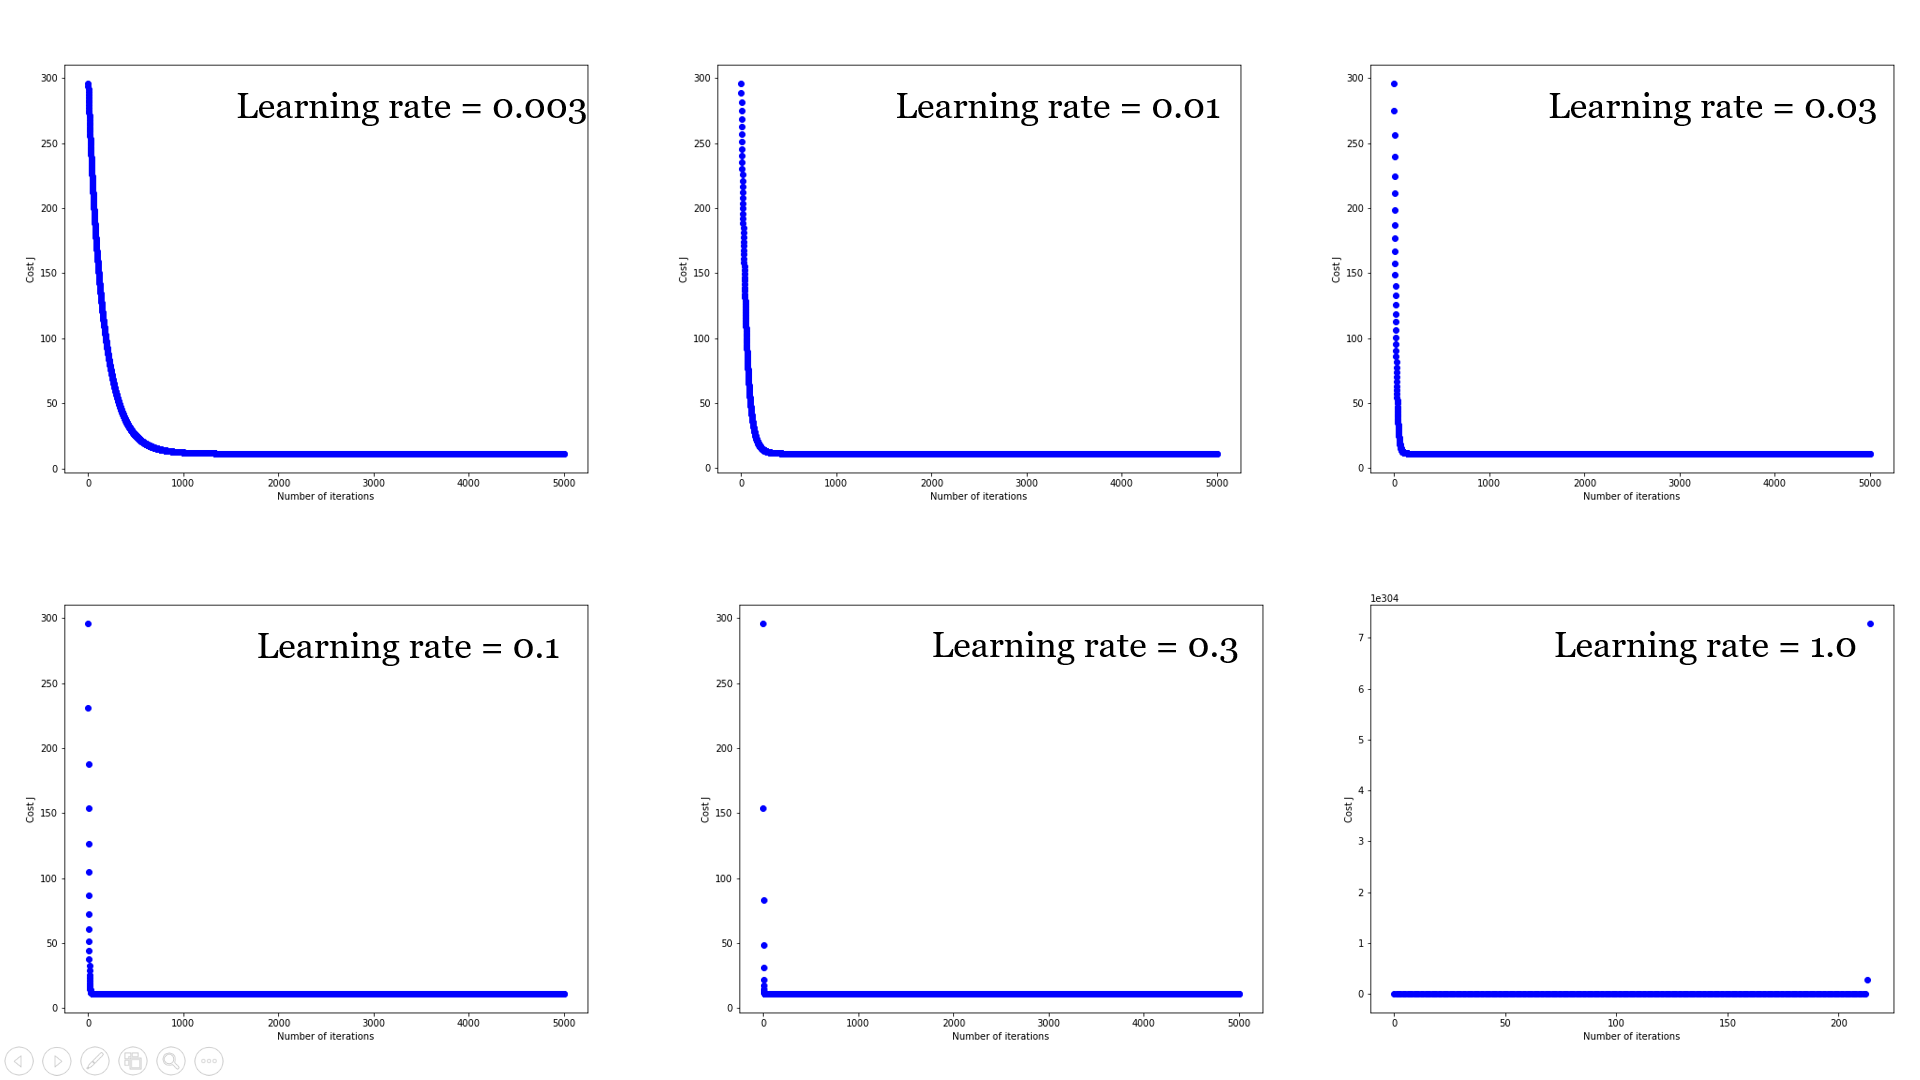
\includegraphics[scale=0.3]{Comparation.png}
         		\caption{learning rates}
         		\label{fig:learningRates}
         	\end{figure}
            \begin{figure}
         		\centering
         		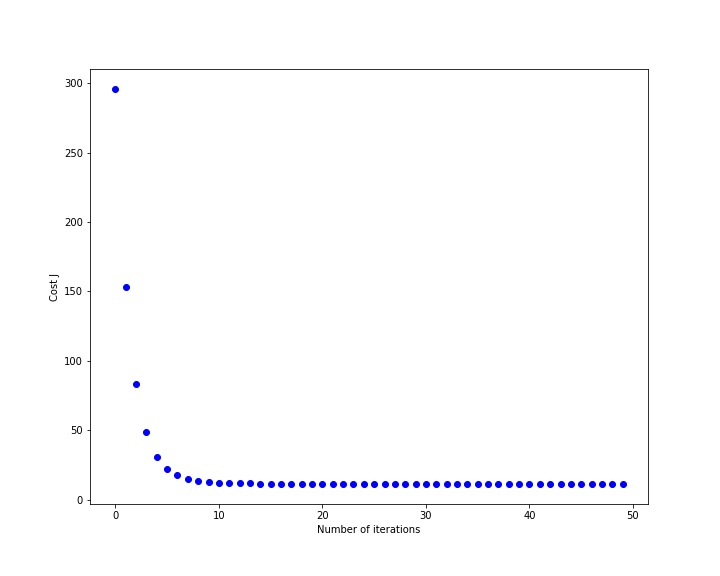
\includegraphics[scale=0.3]{learningRateSpec.png}
         		\caption{learning rates=0.3, scale up x axis}
         		\label{fig:learningRatesSpecific}
         	\end{figure}
         \\ \textbf{Writeup}: As we can see in the Figure \ref{fig:learningRates}, as the learning rate increases, the gradient descent will be faster. However, as it is larger than a threshold, the gradient won't descent any more. Here we find the proper learning rate should be about 0.3. When the learning rate is equal to 0.3, let's scale up the X axis to find the proper number of iterations. As we can see in the Figure \ref{fig:learningRatesSpecific}, the proper number of iterations should be around 10, because the gradient remains unchanged after this point.
\end{itemize}

\paragraph{\textbf{Part 2}}
\begin{itemize}
	\item
        \textbf{Question}: Modify the lambda parameter in the cell above and try $\lambda$=1,10,100. For each of these values, the script will generate a polynomial fit to the data and also a learning curve. Submit two plots for each value of lambda: the fit as well as the learning curve. Comment on the impact of the choice of lambda on the quality of the learned model.
    \\ \textbf{Plots}:
        Figure \ref{fig:modifyLambda} shows the plots for each value of lambda: the fit as well as the learning curve. $\lambda$=0,1,10,100
        \begin{figure}
     		\centering
     		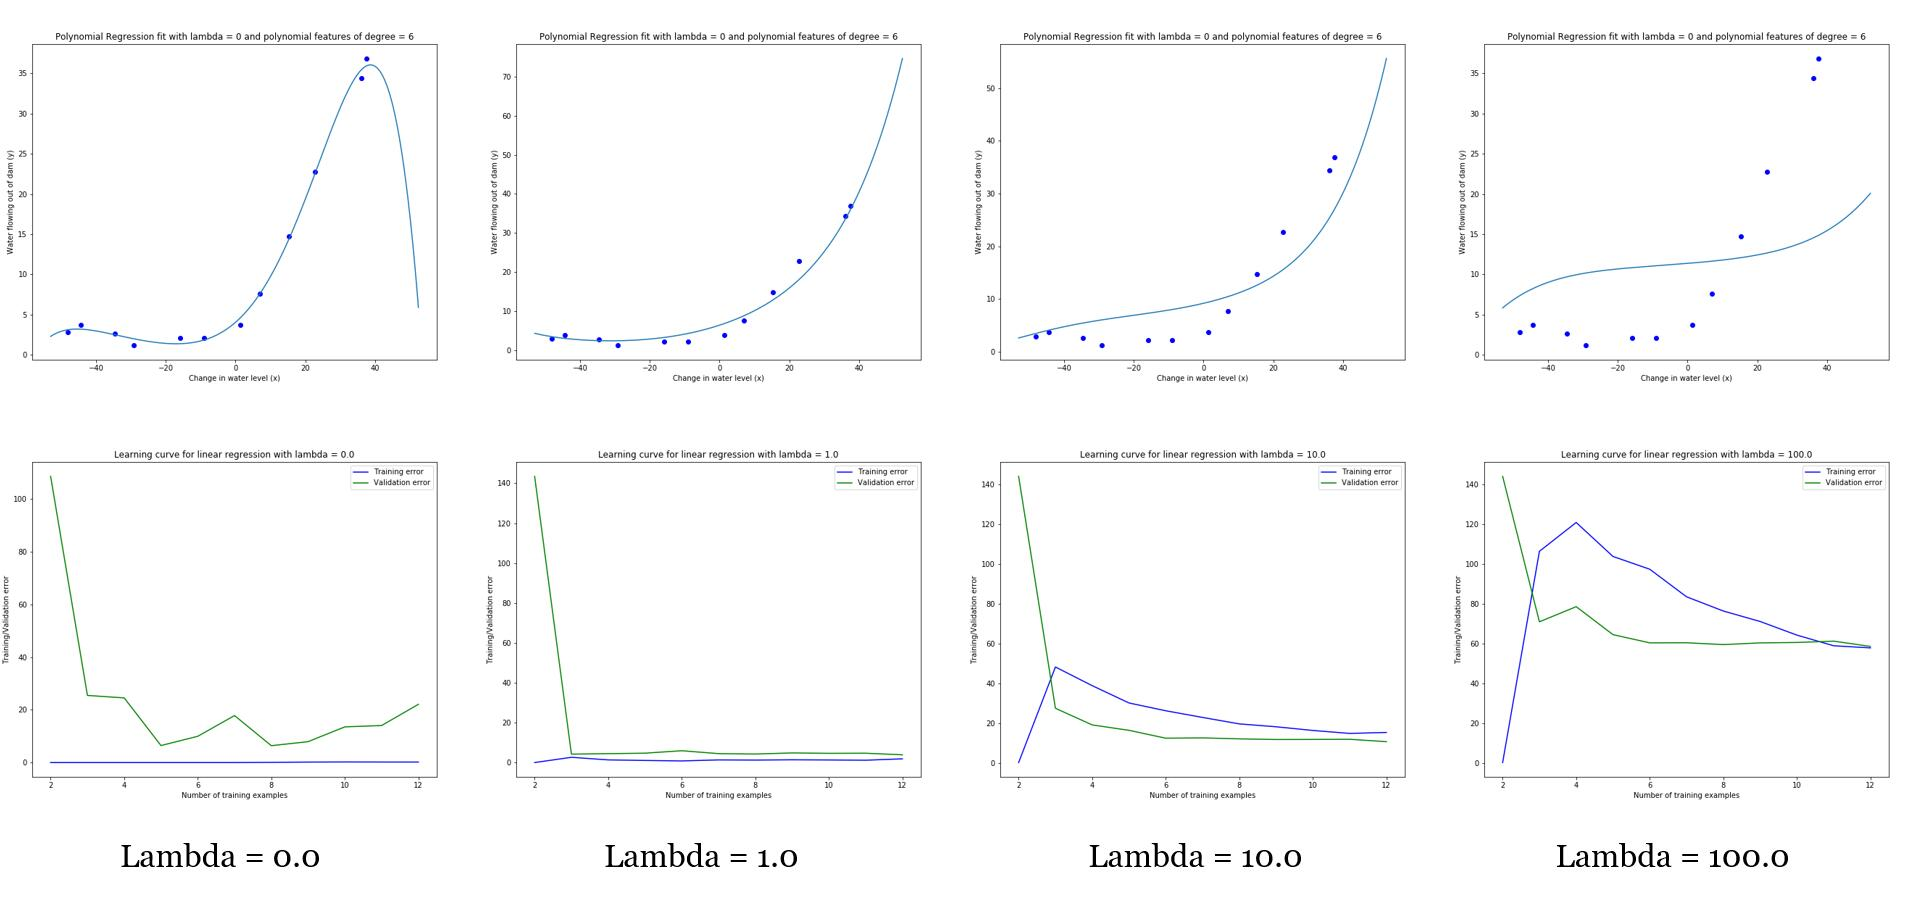
\includegraphics[scale=0.3]{Comparation2.jpg}
     		\caption{modify lambda}
     		\label{fig:modifyLambda}
     	\end{figure}
     \\ \textbf{Comment}: As $\lambda$ becomes larger and larger, the model become more and more inaccurate. But the bias becomes lower, and the variance becomes higher. As we can see from the \ref{fig:modifyLambda}, the most proper $\lambda$ here should be around 1.0. At this point, the model fit the data and the gradient will be convergence.

    \item
        \textbf{Question}: Calculate the error of the best model that you found with the previous analysis and report it.
     \\ \textbf{Answer}:
        \\ when $\lambda=1.0$, then:
        \\Optimization terminated successfully.
         \\ Current function value: 6.891076
         \\ Iterations: 21
         \\ Function evaluations: 22
         \\ Gradient evaluations: 22
         \\ 3.0987482655574246

     \item
        \textbf{Question}: You will implement an automated method to select the $\lambda$ parameter. You should try $\lambda$ in the following range: {0, 0.001, 0.003, 0.01, 0.03, 0.1, 0.3, 1, 3, 10}. Run the cell below to plot a validation curve of $\lambda$ versus the error. Comment on the best choice of $\lambda$ for this problem.
        \\ \textbf{Plot}:
        Figure \ref{fig:validationCurve} shows how training error and validation error change as $\lambda$ increase.
        \begin{figure}
     		\centering
     		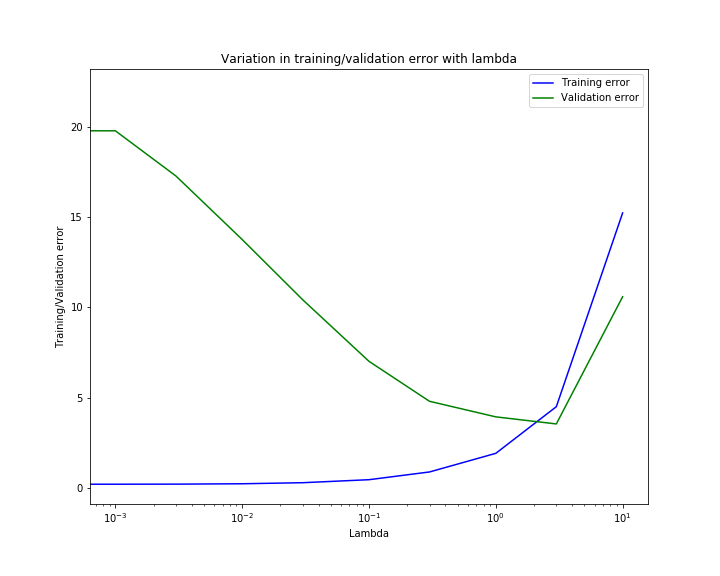
\includegraphics[scale=0.3]{validation_curve.png}
     		\caption{validation curve}
     		\label{fig:validationCurve}
     	\end{figure}
     \\ \textbf{Comment}: Taking the error to be minimum when selecting the $\lambda$, the best $\lambda$ is: 3. When the $\lambda$ is too small, the model tend to be overfit. And when the $\lambda$ is too big, the model tend to be unfit.
\end{itemize}

\paragraph{\textbf{Extra Credit}}
\begin{itemize}
	\item
        \textbf{Question}: What is the lowest achievable error on the test set with $\lambda=0$?
     \\ \textbf{Answer}: Test err of the best linear model with lambda = 0 is: 14.558424000416249.

     \item
        \textbf{Question}:  Select the best value for $\lambda$ and report the test set error with the best $\lambda$?
    \\ \textbf{Plot}:
        Figure \ref{fig:extraCredit1} shows the training and validation error with different $\lambda$.
        \begin{figure}
     		\centering
     		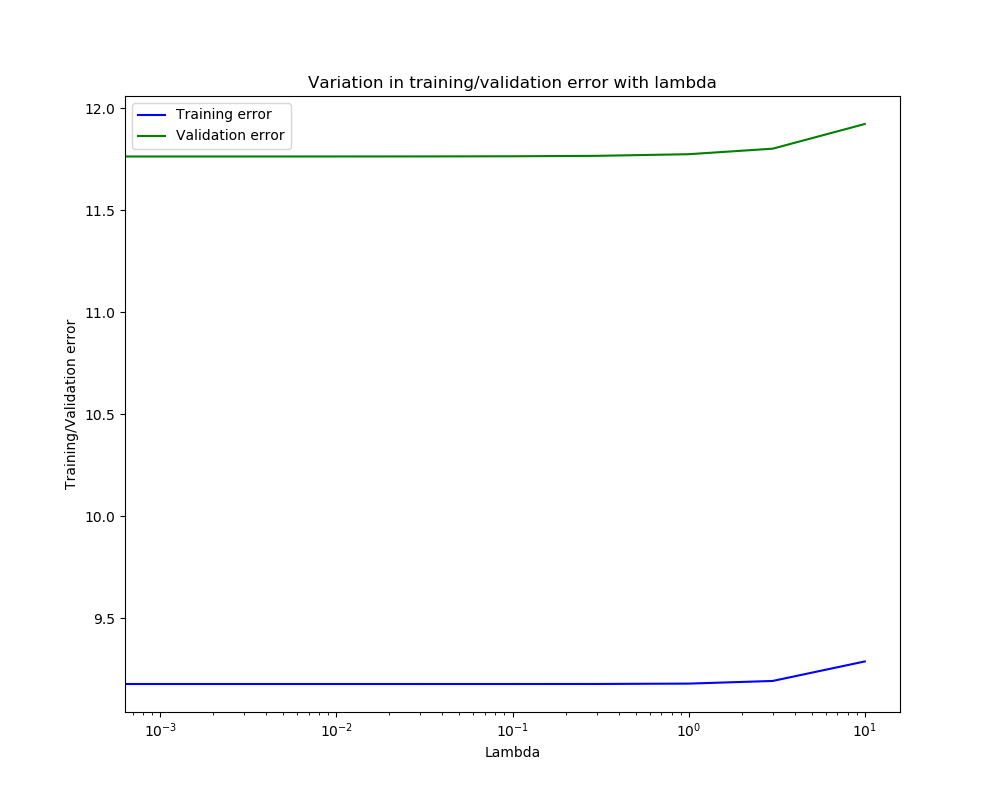
\includegraphics[scale=0.3]{liner.png}
     		\caption{modify lambda}
     		\label{fig:extraCredit1}
     	\end{figure}
     \\ \textbf{Answer}: As we can see from the \ref{fig:extraCredit1}, the best value for $\lambda$ is 0. At this time, the lowest achievable error is 14.558424000416249.

     \item
        \textbf{Question}:  Use the technique of adding features to extend each column of the Boston data set with powers of the values in the column. Repeat the bias-variance analysis with quadratic and cubic features. What is the test set error with quadratic features with the best $\lambda$ chosen with the validation set? What is the test set error with cubic features with the best $\lambda$ chosen with the validation set?
    \\ \textbf{Plot}:
        Figure \ref{fig:extraCredit2} shows the training and validation error with different $\lambda$ when it comes to use the technique of adding features with quadratic, and with cubic features.
        \begin{figure}
     		\centering
     		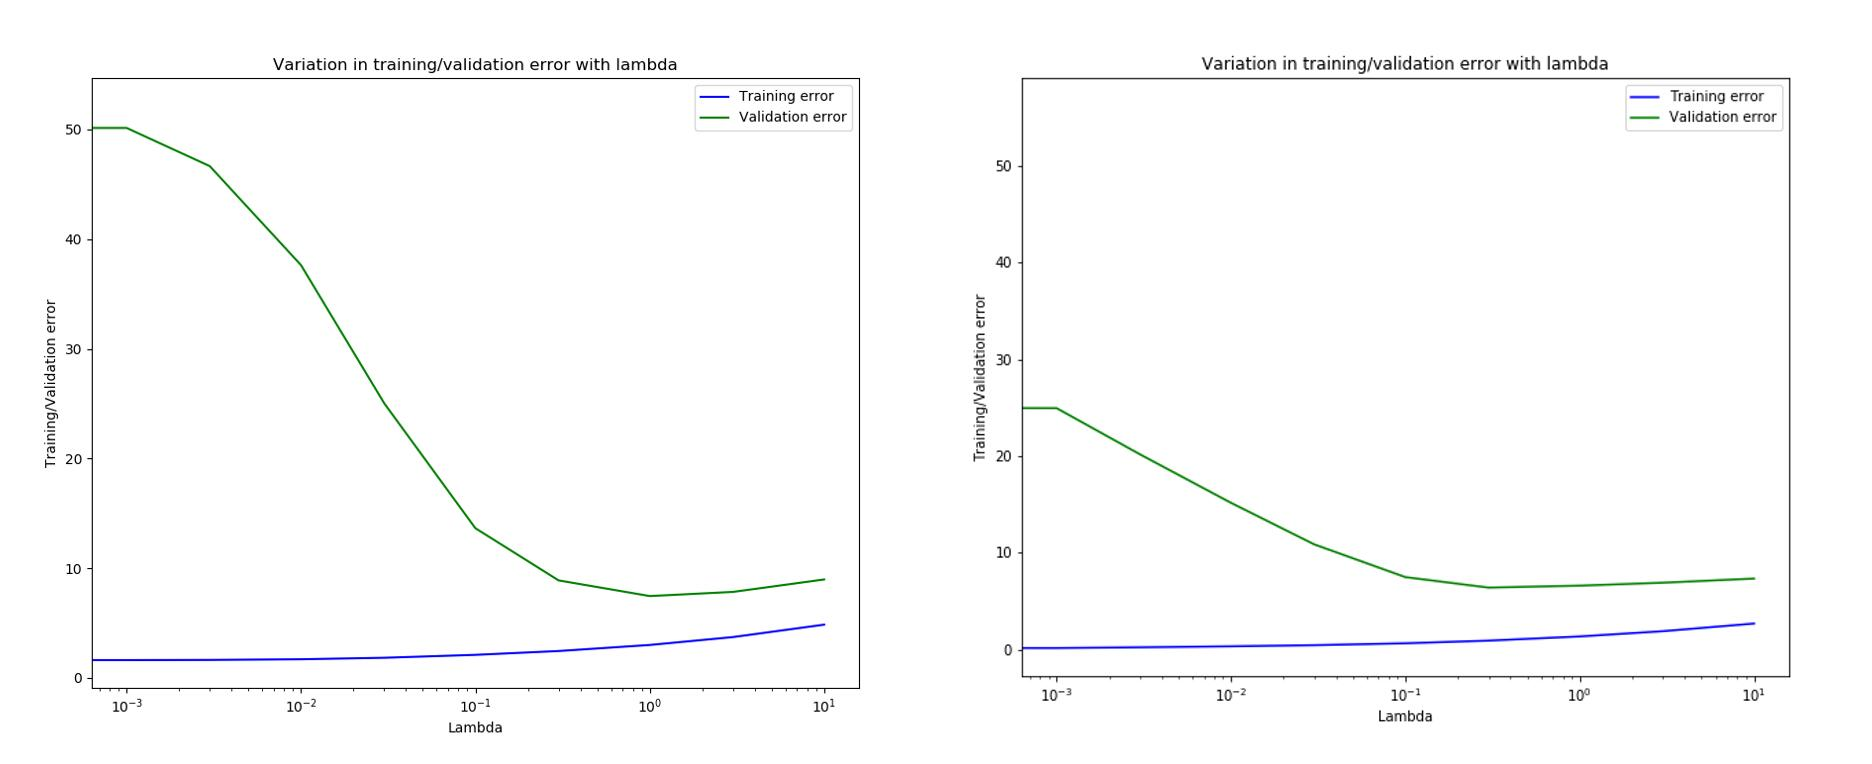
\includegraphics[scale=0.25]{Comparation5.jpg}
     		\caption{modify lambda, with quadratic features (left), and with cubic features (right)}
     		\label{fig:extraCredit2}
     	\end{figure}
     \\ \textbf{Answer}:
        \begin{itemize}
            \item When it comes to use quadratic features, the best lambda is: 1, and minimum error value is: 5.5471436479140115.
            \item When it comes to use cubic features, the the best lambda is: 0.3, and minimum error value is: 7.7848111200607555.
        \end{itemize}

     \item
        \textbf{Question}: Discuss the impact of regularization for building good models for the Boston housing data set.
        \\ \textbf{Answer}: Regularization allows complex models to be trained on data sets of limited size without severe overfitting, essentially by limiting effective model complexity.
\end{itemize}

\end{document}

